\documentclass[a4paper,12pt, english]{article}
\usepackage[T1]{fontenc}
\usepackage[utf8]{inputenc}
\usepackage{graphicx}
\usepackage{babel}
\usepackage{amsmath}
\usepackage{ulem}
\usepackage{a4wide}
\usepackage{graphicx}
\usepackage{listings}
\usepackage{tabularx}
\usepackage{tabulary}

\begin{document}

\begin{titlepage}
\begin{center}
\textsc{\Large Computational Physics, Project 3}\\[0.5cm]
\textsc{Vilde Eide Skingen and Kari Eriksen}\\[0.5cm]

\end{center}
\end{titlepage}

\begin{abstract}
The aim of project 3 is to create a code for simulating the solar system. In the first part we will look at a hypothetical solar system consisting of the Sun and the Earth. We will assume that the Sun's mass is sufficiently large, so that its motion can be neglected. With this assumption we will compute the motion of the Earth using the Runge-Kutta solver to solve an ordinary differential equations. Later we will add several other planets to our simulation, and see how the forces between the objects effects the individual orbits.   
\end{abstract}

\section*{A model for the solar system}

\subsection*{Introduction}
In the first part of the project our goal is to calculate the position of Earth as a function of time. The only force in the project is the gravitational force between the heavenly bodies. We first look at a hypothetical solar system consisting only of the Earth and the Sun. However, we will write our program in such a way that it is easy to add other planets in our simulation. 

\subsection*{Theory}

In the first part of the project we will look at a hypothetical solar system with only one planet, the Earth, in orbit around the Sun. The only force in this problem is gravity, given by Newton's law of gravitation $$ F_G = \frac{GM_{sun}M_{Earth}}{r^2} $$
where $M_{sun}$ and $M_{Earth}$ are the masses of the Sun and Earth, $r$ the distance between them, and $G$ the gravitational constant. If we assume that the Sun has a much larger mass than the mass of the Earth, we can safely neglect the motion of the sun in the calculations. 

We will also assume that the orbit of Earth around the Sun is co-planar, and that it lies in the $xy$-plane. We  then get the following equations from Newton's second law of motion
$$\frac{d^2x}{dt^2} = \frac{F_{G,x}}{M_{Earth}}$$
$$\frac{d^2y}{dt^2} = \frac{F_{G,y}}{M_{Earth}}$$
where $F_{G,x}$ and $F_{G,y}$ are the $x$ and $y$ component of the gravitational force. 


\begin{figure}[h!]
  \centering
    	  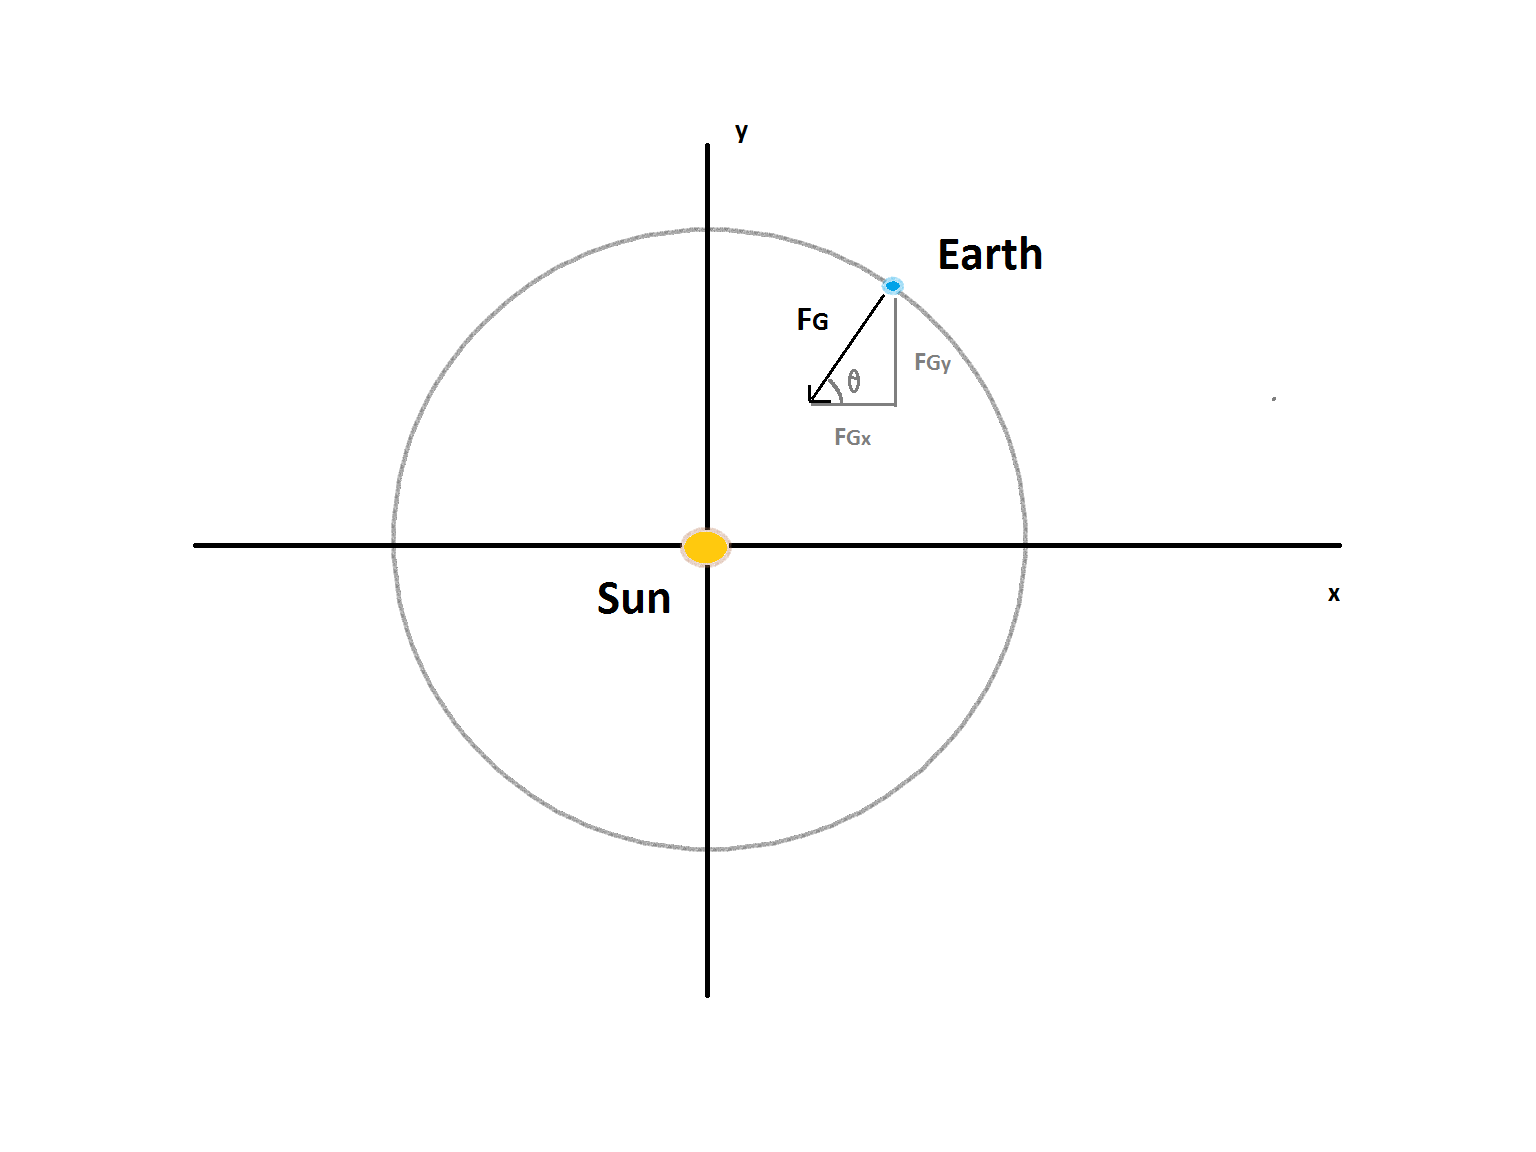
\includegraphics[scale=0.4]{project3.png}
  \caption{\textit{Coordinate system with the Sun at the center and Earth located at (x,y) in orbit around the Sun}}
\end{figure}


From figure 1 we have that

$$F_{G,x} = - F_G  \hspace{0.7 mm} cos \theta = - \frac{GM_{sun}M_{Earth}}{r^2} \hspace{0.7 mm} cos \theta $$
$$F_{G,y} = - F_G \hspace{0.7 mm} sin \theta = - \frac{GM_{sun}M_{Earth}}{r^2} \hspace{0.7 mm} sin \theta $$


\begin{figure}[h!]
  \centering
    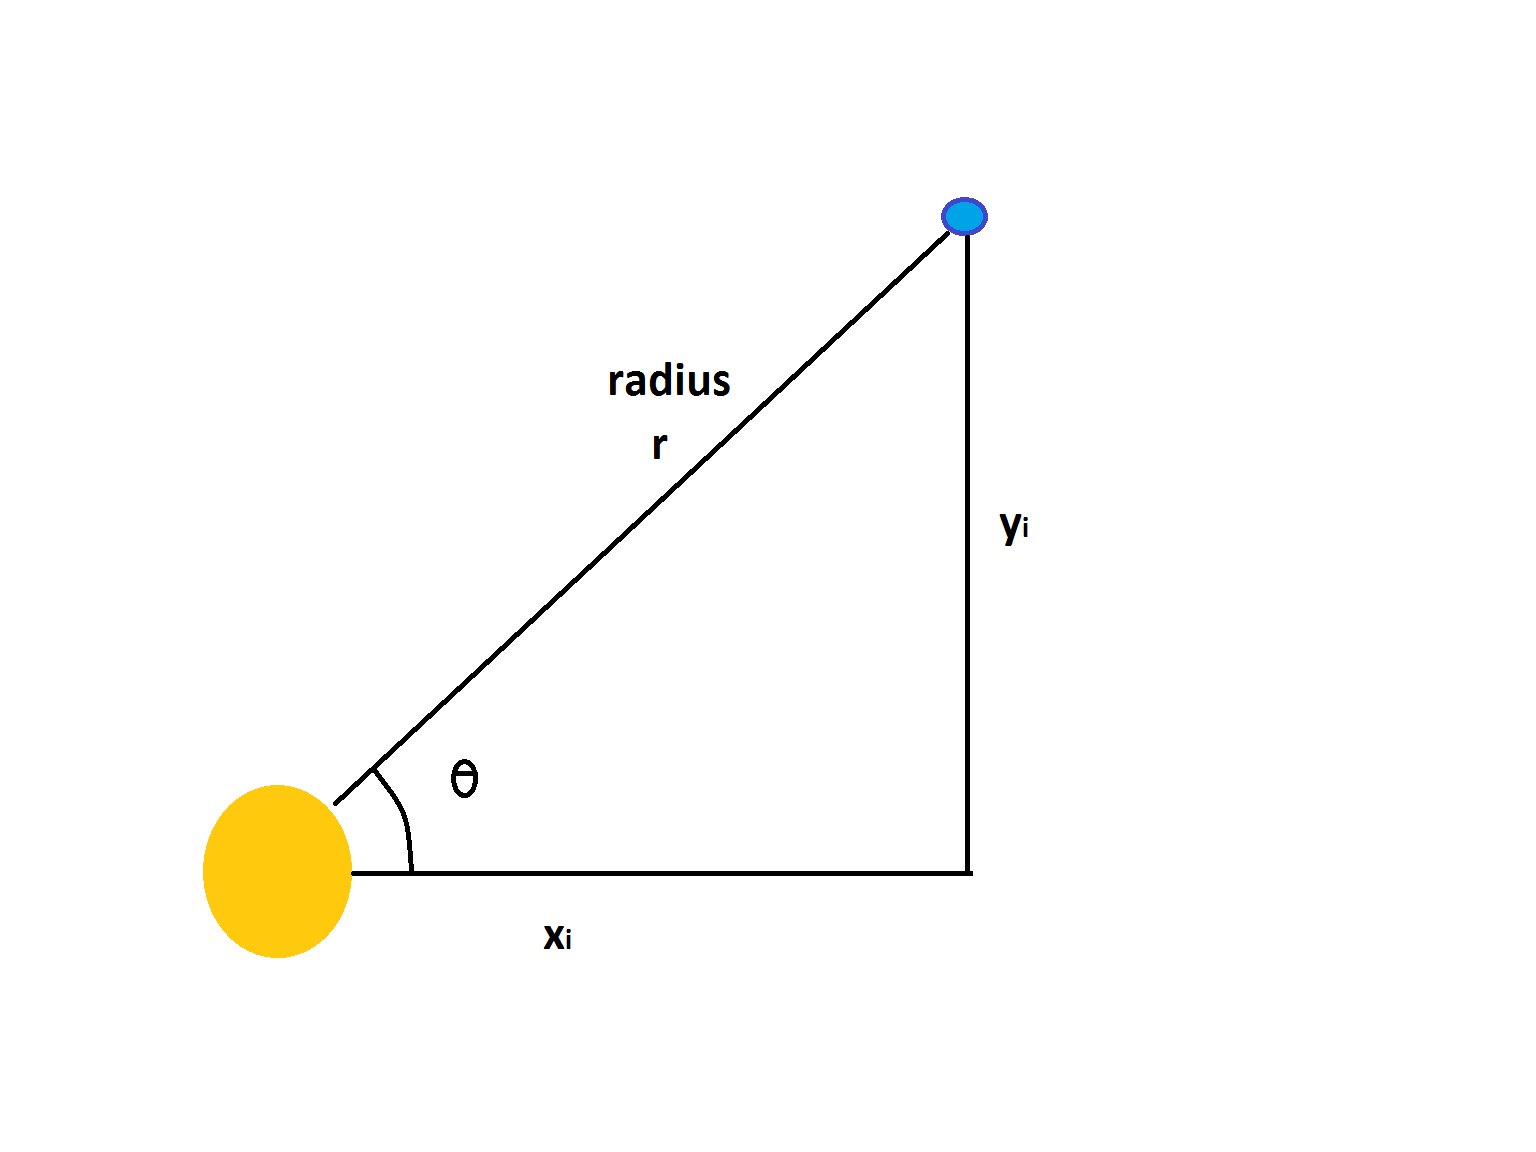
\includegraphics[scale=0.2]{project3_1.png}
  \caption{\textit{Relation between the distance between Earth and the Sun and the angle $\theta$}}
\end{figure}

and figure 2 gives that

$$ cos \theta = \frac{x_i}{r} $$
$$ sin \theta = \frac{y_i}{r} $$

We can rewrite the second-order ordinary differential equations as a set of coupled first order differential equations. 
We know that the velocity is connected to the position by the time derivative so that
$$ \frac{dx}{dt} = v_x \hspace{20 mm} \frac{dy}{dt} = v_y$$
and thus we have that
$$ \frac{dv_x}{dt} = \frac{F_{G,x}}{M_{Earth}} \hspace{20 mm} \frac{dv_y}{dt} = \frac{F_{G,y}}{M_{Earth}} $$

These ordinary differential equations can be solved by numerical methods. However, before doing so, we should find a suitable choice of units. We choose to use the astronomical units in our project. The astronomical unit of length is given to be the average distance between the Sun and the Earth, $1 AU = 1.5*10^{11} m$. It is convenient to measure time in years, since this better suits the cycles of the solar system. We choose to measure mass relative to the Sun's mass.

In preparation of constructing a computational solution, we convert the equations of motion into a discretized set of equations. The acceleration is given by Newton's second law, $$ F = ma $$. The change in velocity is $a \Delta t$, and the change in position is $v \Delta t$. Thus we find the q
equations for the Earth effected by the gravitational force from the Sun to be

$$v_{x,i+1} = v_{x,i} - \frac{G M_{sun} x_i}{r_i ^3} \hspace{0.5mm} \Delta t $$ 
$$x_{i+1} = x_i + v_{x,i+1} \Delta t $$
$$v_{y,i+1} = v_{y,i} - \frac{G M_{sun} y_i}{r_i ^3} \Delta t $$
$$y_{i+1} = y_i + v_{y,i+1} \Delta t $$


where $\Delta t$ is the time step. In the case of circular orbit we have that $4 \pi ^2 = GM_{sun}$.

For circular motion we know that the force must obey the following relation 
$$\frac{M_{Earth}v^2}{r} = F_G = \frac{GM_{sun}M_{Earth}}{r^2}$$ where $v$ is the velocity of the Earth. 
For circular orbit the velocity of the Earth is $v = \frac{2 \pi r}{1 year}$, where the distance between Sun and Earth is $r = 1 AU$. Hence $v = 2 \pi (AU/years)$. Rearranging the equation we find
$$v^2r = GM_{sun} = 4 \pi ^2 AU^3/years^2$$

For circular motion the velocity will be tangential. It follows that if we choose the initial conditions $ x = 1 AU $ and $ y = 0$, with velocities $v_x = 0$ and $v_y = v_{tangential} = 2 \pi AU/year$ we will get a circular orbit.  


\subsection*{Method}
To compute the trajectories of the different astronomical objects we made a vector $A$ that holds information of the initial position and velocity in x and y direction for all objects. That is our vector $A$ is a $4*n$ vector, where $n$ is the number of objects.

\[ A = \left( \begin{array}{c}
x - object 1\\
y - object 1\\
vx - object 1\\
vy -object 1\\
x - object 2\\
... \\
vy - object n \end{array} \right)\]   

We computed the time derivative of this vector and saved it in a vector $dAdt$. The derivative of the position equals the velocity, so these values we could read directly from our $A$ vector. 
To find the acceleration, the time derivative of the velocities, we computed the radius between the different objects, and calculated the force between them. By using Newton's second law we found the acceleration of each object. We then used these values in the Runge-Kutta 4 scheme to make estimates of the next positions and velocities. For each time step we wrote the $x$ and $y$ values to a file so that we could make plots of the objects trajectories.    

The Runge-Kutta solver is a method for solving ordinary differential equations for which we know the initial values. In this project the motion of the planets are described by a second-order differential equation of the position as a function of time. We want to find the propagation of this function forward in time starting from the given initial values. 

Taylor series expansion of a function $x$ around $t$ gives
$$ x(t+ \Delta t) = x(t) + \frac{dx}{dt} \Delta t + \frac{1}{2} + \frac{d^2 x}{d^2 t} (\Delta t)^2 + \cdots $$

If we assume a reasonable smooth function $x(t)$ and a small interval $\Delta t$ we can approximate $x(t)$ to $x(t + \Delta t)$ as long as we know the derivatives of $x(t)$. 
When using the Runge-Kutta approximation one estimates the slopes at four points, once at the initial point, twice at the trial midpoint and once at the trial endpoint. 
$$ k_1 = \Delta t f(t_i,x_i) \\
k_2 = \Delta t f(t_i + \Delta t /2, x_i + k_1/2) \\
k_3 = \Delta t f(t_i + \Delta t/2, x_i + k_2/2) \\
k_4 = \Delta t f(t_i + \Delta t, x_i + k3) $$

These four derivatives constitute the next value in our propagation
$$x_{i+1} = x_i + \frac{1}{6} (k_1 + 2(k_2+k_3) + k_4$$


\subsection*{Results}
When running our program for the two-body system of the Earth and the Sun and for the initial values we in theory predicted to be circular we found that our program lives up to our expectations. Figure somethingsomething.

\begin{figure}[h!]
  \centering
    \includegraphics[scale=0.5]{circular orbit earth.png}
  \caption{\textit{Circular orbit of the Earth only effected by the gravitational force from the Sun}}
\end{figure}


Changing the initial velocity of the Earth....
When we increase the initial velocity the orbit will be elliptical until we reach a high enough velocity for the world to escape it's orbit around the Sun. Figure ... we see the elliptical orbit.  

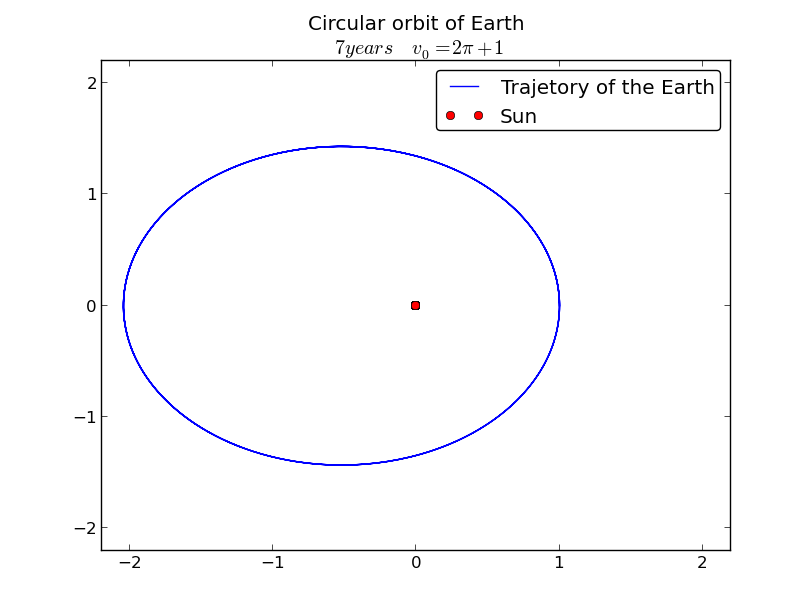
\includegraphics[scale=0.5]{circular_orbit_1.png}
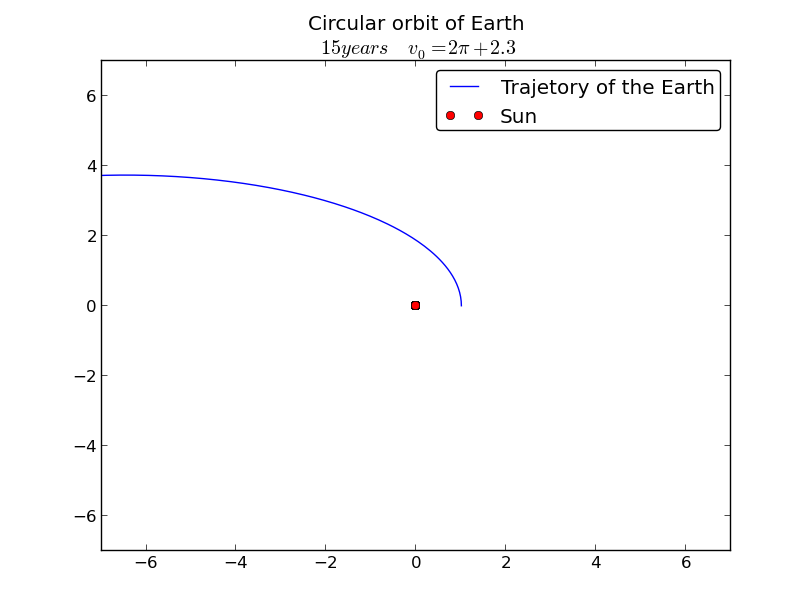
\includegraphics[scale=0.5]{circular_orbit_2.png}

If instead we give a initial velocity "suitable" less then the initial velocity of the circular orbit, the Earth will be dragged towards the Sun. When it get passe close the force from the Sun on Earth will be to big for our program to handle, and thus it looks like the Earth is sent out and escapes the gravitational force working on it.     

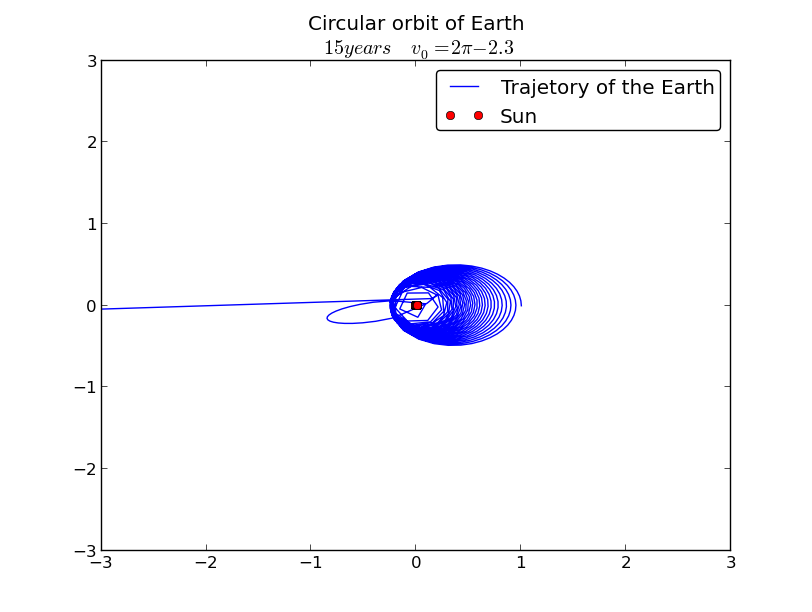
\includegraphics[scale=0.5]{circular_orbit_3.png}

Our algorithm is not stable for large timesteps either. When looking at the initial velocity that should give us circular motion, the program will not yield the wanted result if we don't choose the right timestep. Here for $N = 20, t_f = 2$ and the initial velocity for circular motion.  
The Earth will move towards the Sun. Forces will get to large for our solver to manage --> distance Earth - Sun will go to infinity.
 
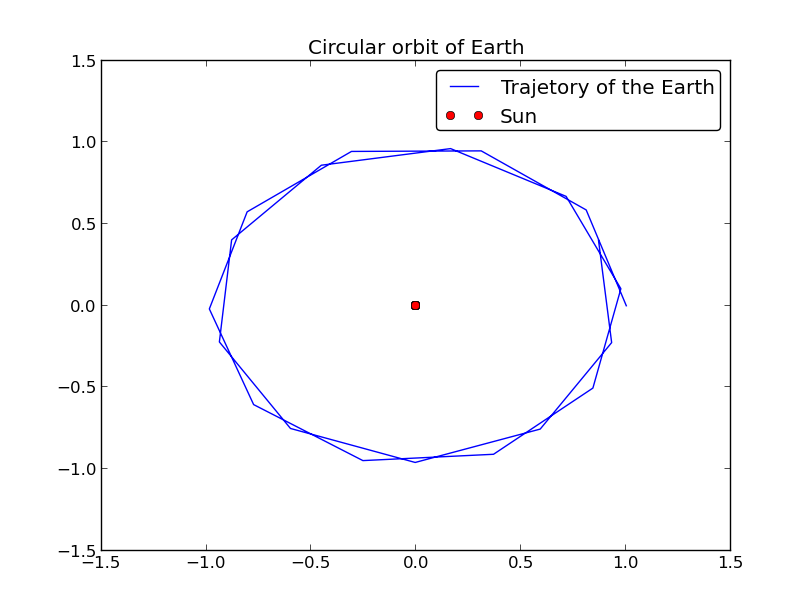
\includegraphics[scale=0.5]{timesteps_circular.png}

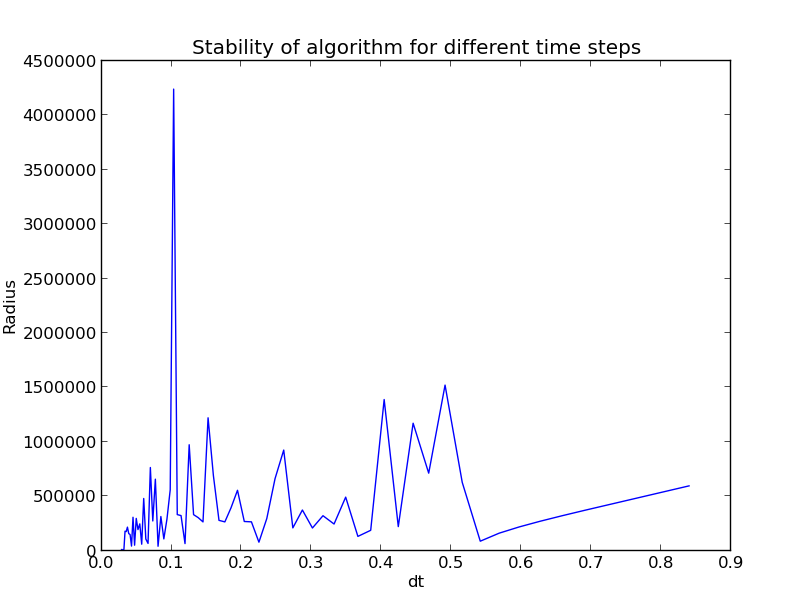
\includegraphics[scale=0.5]{timesteps_stability.png}

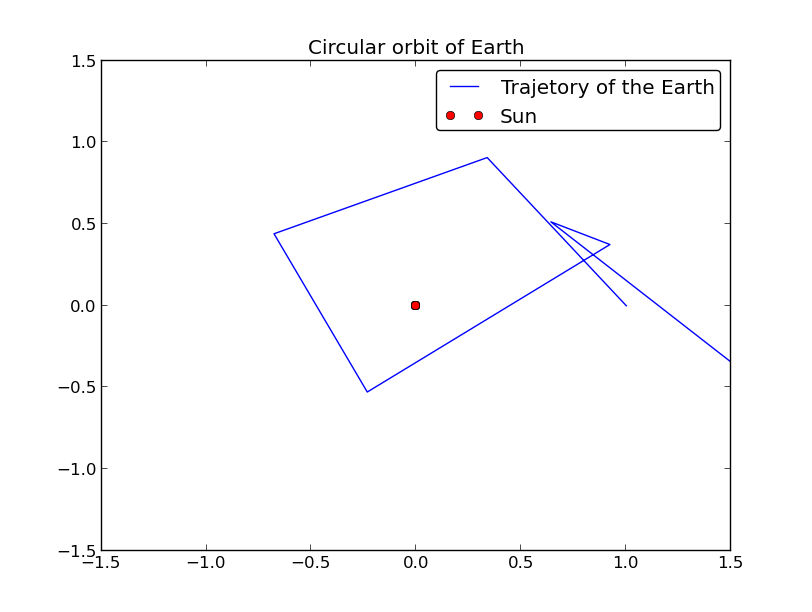
\includegraphics[scale=0.5]{timesteps_stability2.png}

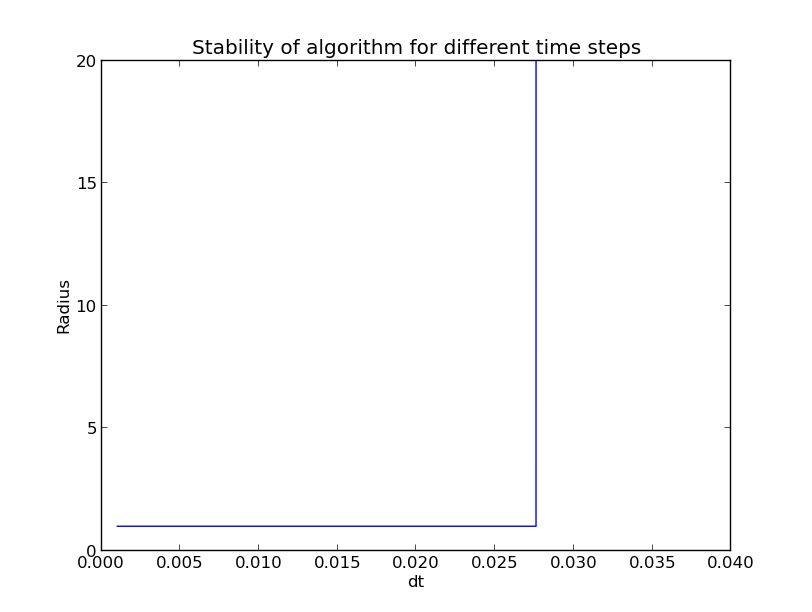
\includegraphics[scale=0.5]{timestep_stability3.png}


Smaller values of delta t give smaller errors (if we ignore the possibility of round-off errors), but reducing delta t leads to a greater computational cost.
Adaptive methods
In case the function to integrate varies slowly or fast in different integration domains,
adaptive methods are normally used. One strategy is always to decrease the step size.
As we have seen earlier, this leads to more CPU cycles and may lead to loss or
numerical precision. An alternative is to use higher-order RK methods for example.
However, this leads again to more cycles, furthermore, there is no guarantee that
higher-order leads to an improved error
\end{document}    